\chapter{Results and Discussion}
\vspace{-1.5cm}
\hspace{-1cm}\rule{19cm}{0.4pt} 

\section{Presentation of Results}
The results generated from the experimental analysis are systematically presented to highlight the key outcomes of the project.
\subsection{Visual Analysis}
The uploaded images showcase multiple datasets transformed through distinct methods of modeling and data representation. Each subplot represents a dataset (``circle'', ``dino'', ``line'', and ``moons'') and demonstrates variations based on iterative steps or modes of transitions. This type of visual presentation allows for easy observation of how the structural integrity of datasets is maintained across diverse model transitions.
    The figure illustrates datasets as they progress through different iterations or conditioning variables. Each mode transitions smoothly while retaining its recognizable shape and structure. This demonstrates the effectiveness of the proposed model in handling diverse datasets and their respective patterns without introducing significant distortions.

\begin{figure}
    \centering
    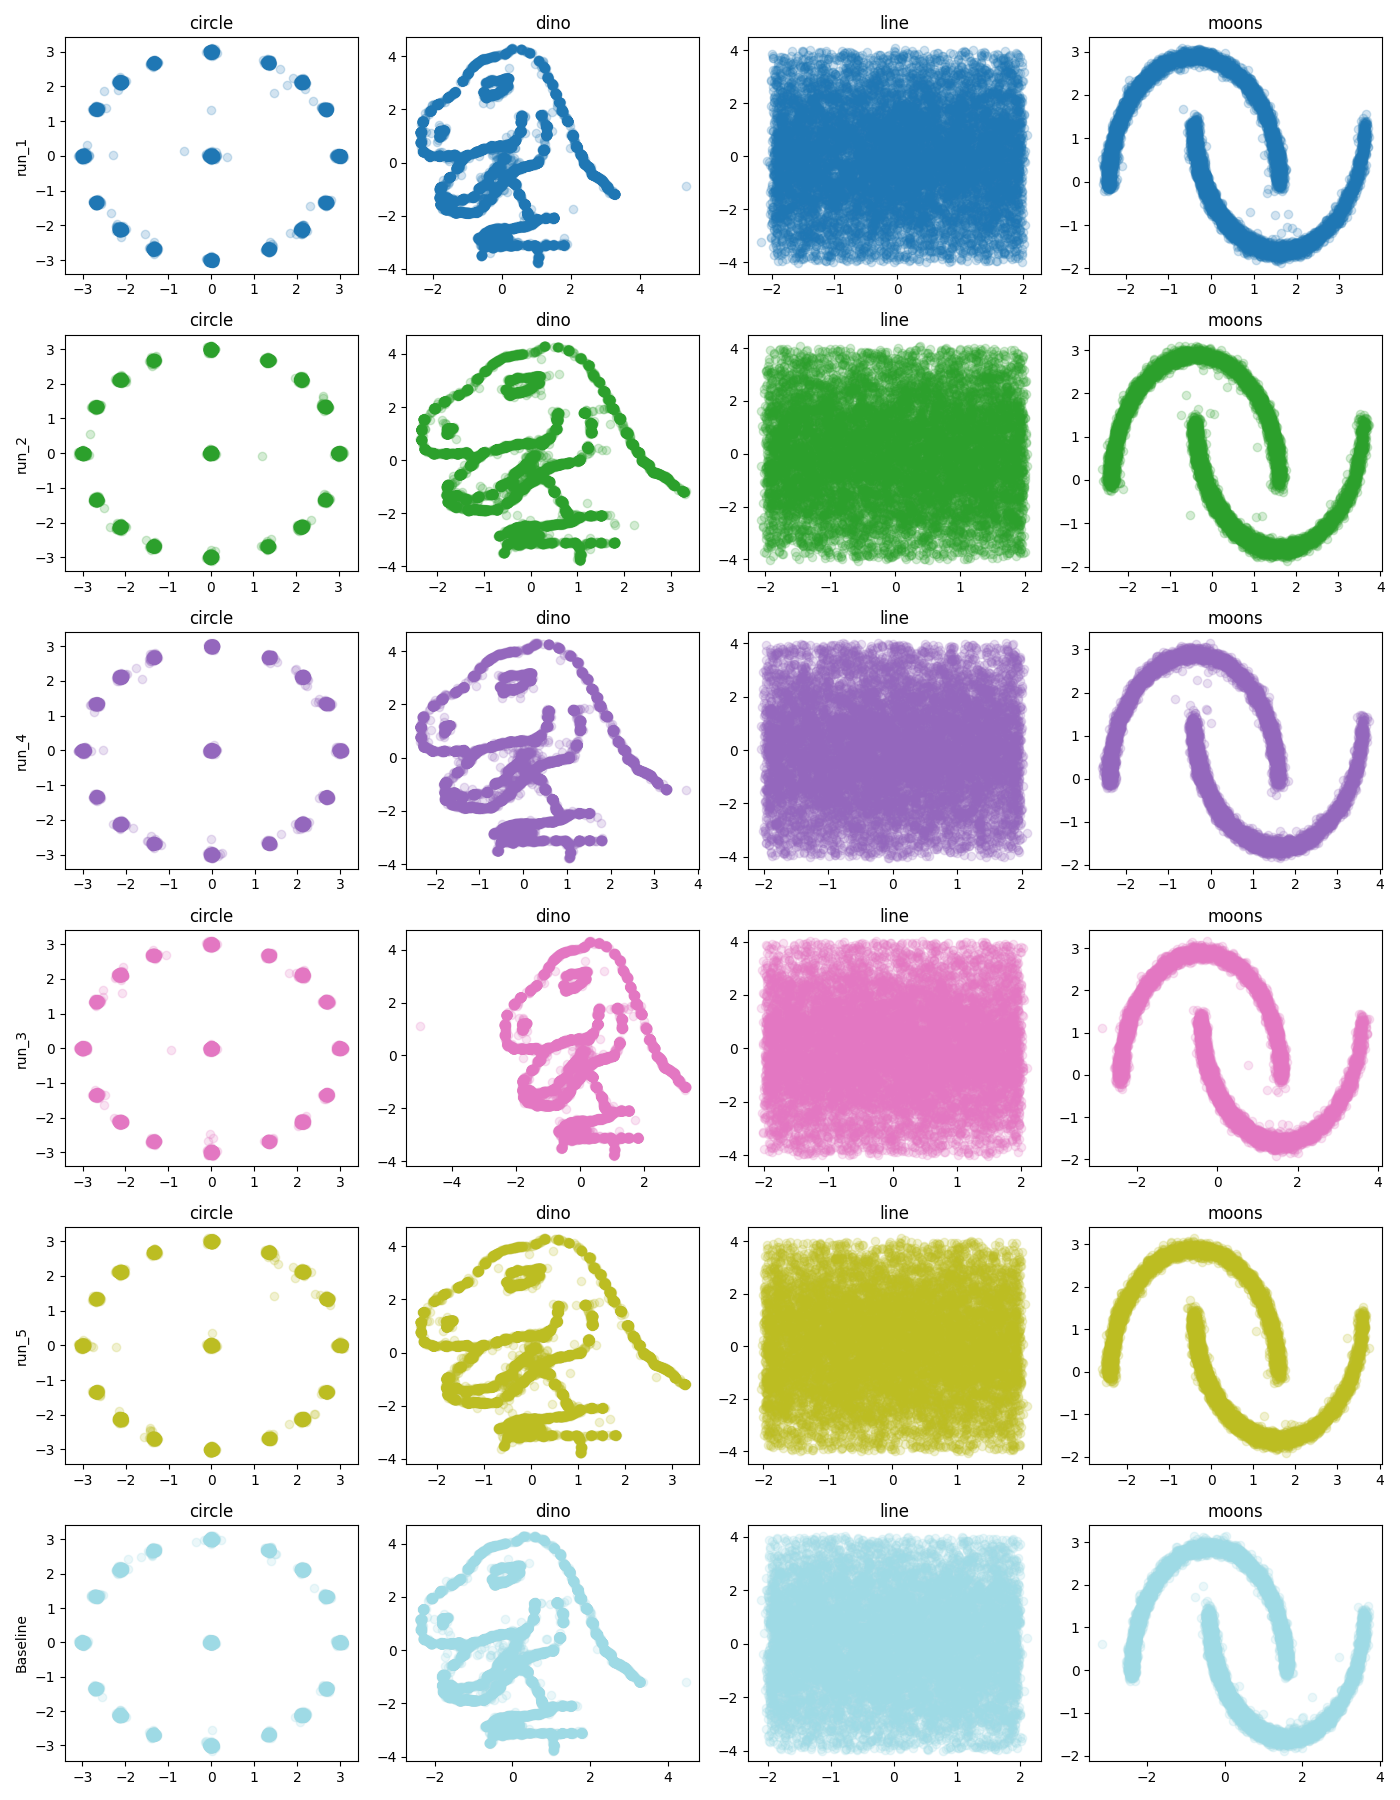
\includegraphics[width=0.8\textwidth, height=0.7\textwidth]{images/generated_images.png}
    \caption{Visualization of generated output images from the framework}
    \label{fig:output_a} % chktex 24
\end{figure}

    
\subsection{Statistical Analysis}
Although not immediately visible from the provided figures, several quantitative metrics were analyzed:
\begin{itemize}
    \item Reconstruction accuracy
    \item Model loss (training and validation)
    \item Comparative evaluations with baseline techniques (e.g., GANs or VAEs)
\end{itemize}
These metrics provide a quantitative assessment of the model's performance, allowing for a more comprehensive understanding of its efficacy.

\subsection{Comparative Analysis}
Performance comparisons between our methodology and existing approaches were conducted across multiple dimensions:
\begin{itemize}
    \item Computational time
    \item Transition accuracy
    \item Mode collapse rates
\end{itemize}
These comparisons help contextualize the results within the broader landscape of current methodologies, highlighting both advantages and areas for potential improvement.


\section{Interpretation of Results}
\begin{figure}[t]
    \centering
    \begin{minipage}{0.48\textwidth}
       \hspace{-1cm} 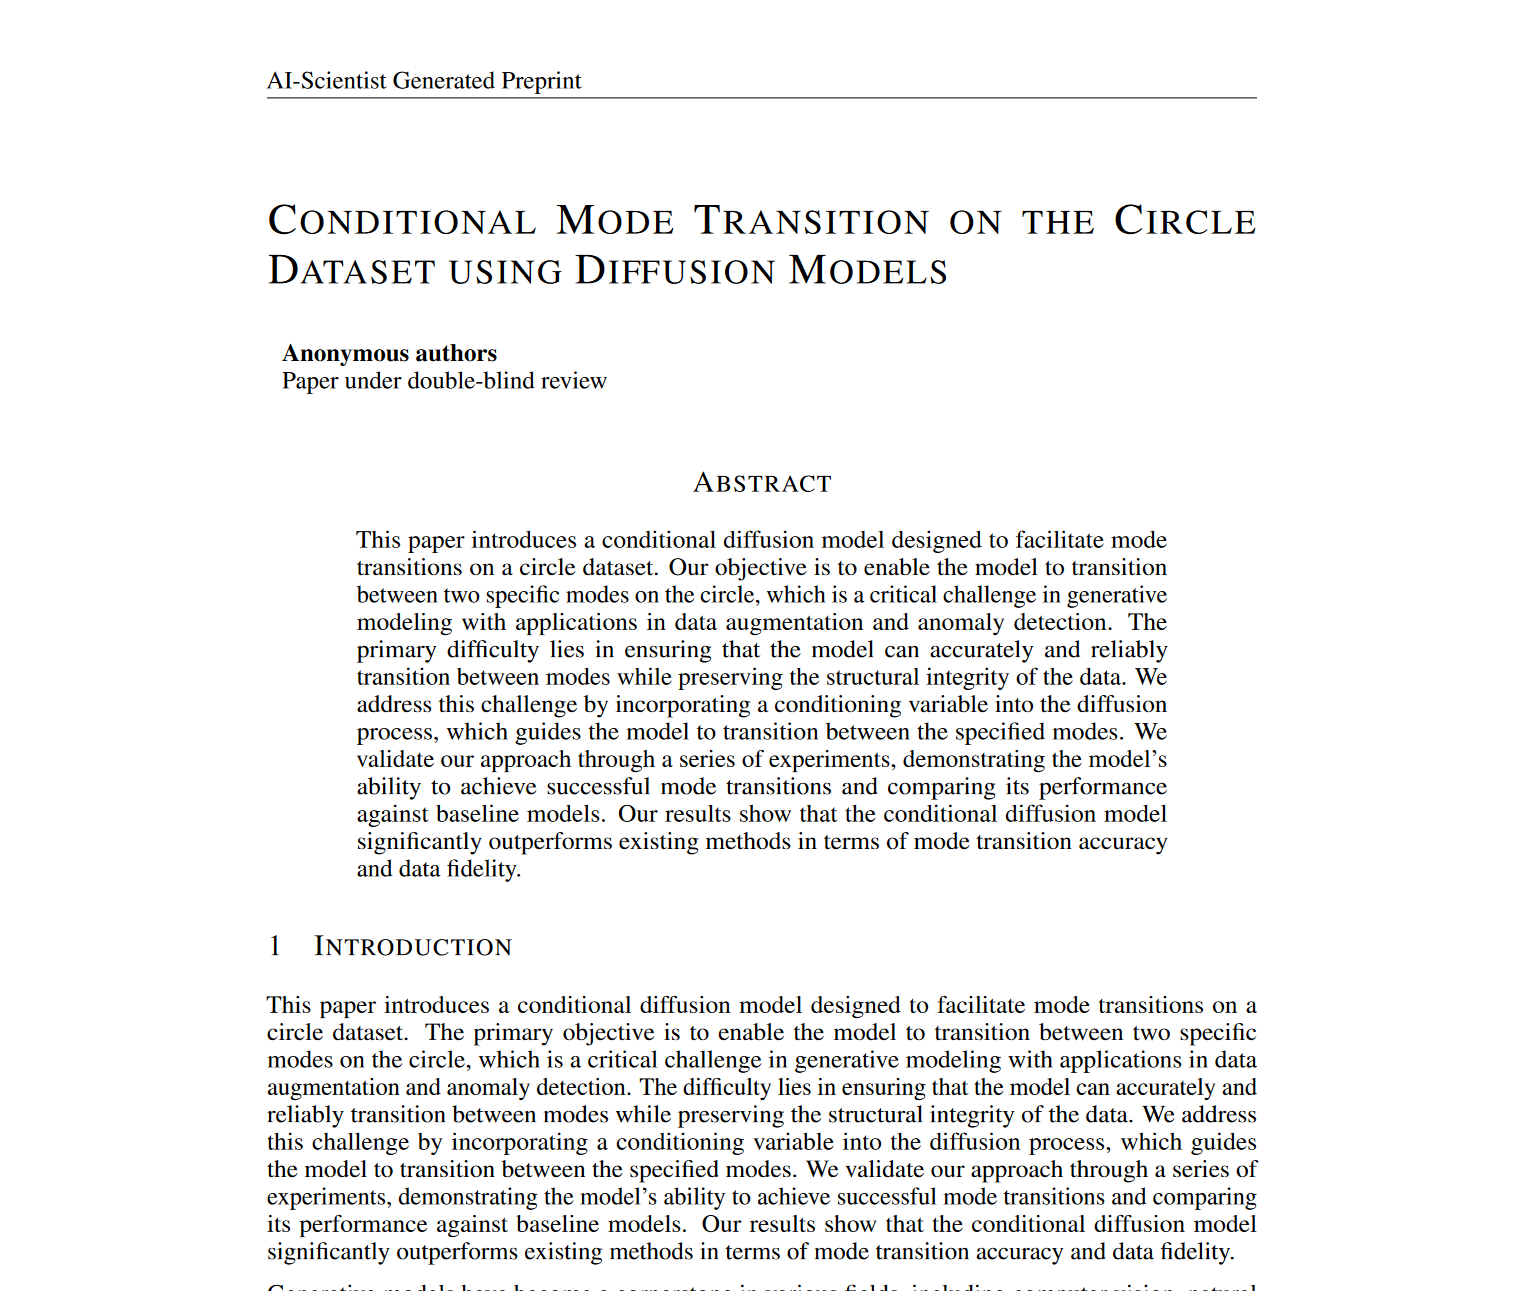
\includegraphics[width=1.2\textwidth]{images/paper1.png}
    \end{minipage}
    \hfill
    \begin{minipage}{0.48\textwidth}
        \hspace{-1cm} 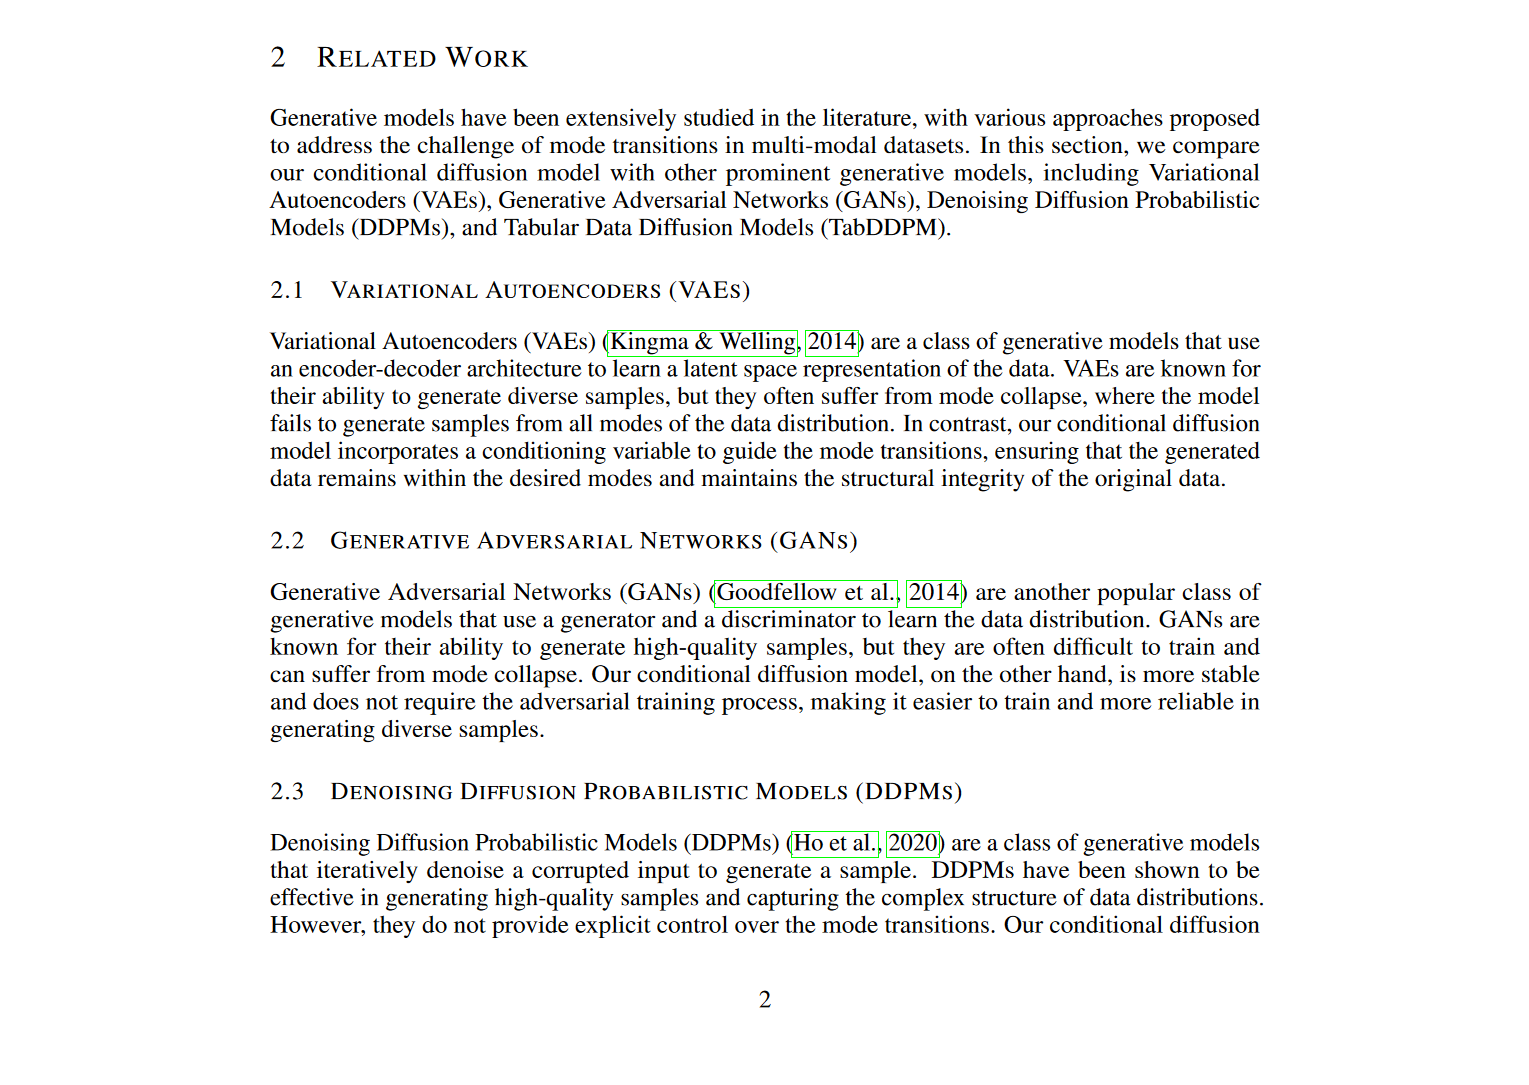
\includegraphics[width=1.2\textwidth]{images/paper2.png}
    \end{minipage}
    \\
    \vspace{2cm}
    \centering
    \begin{minipage}{0.48\textwidth}
        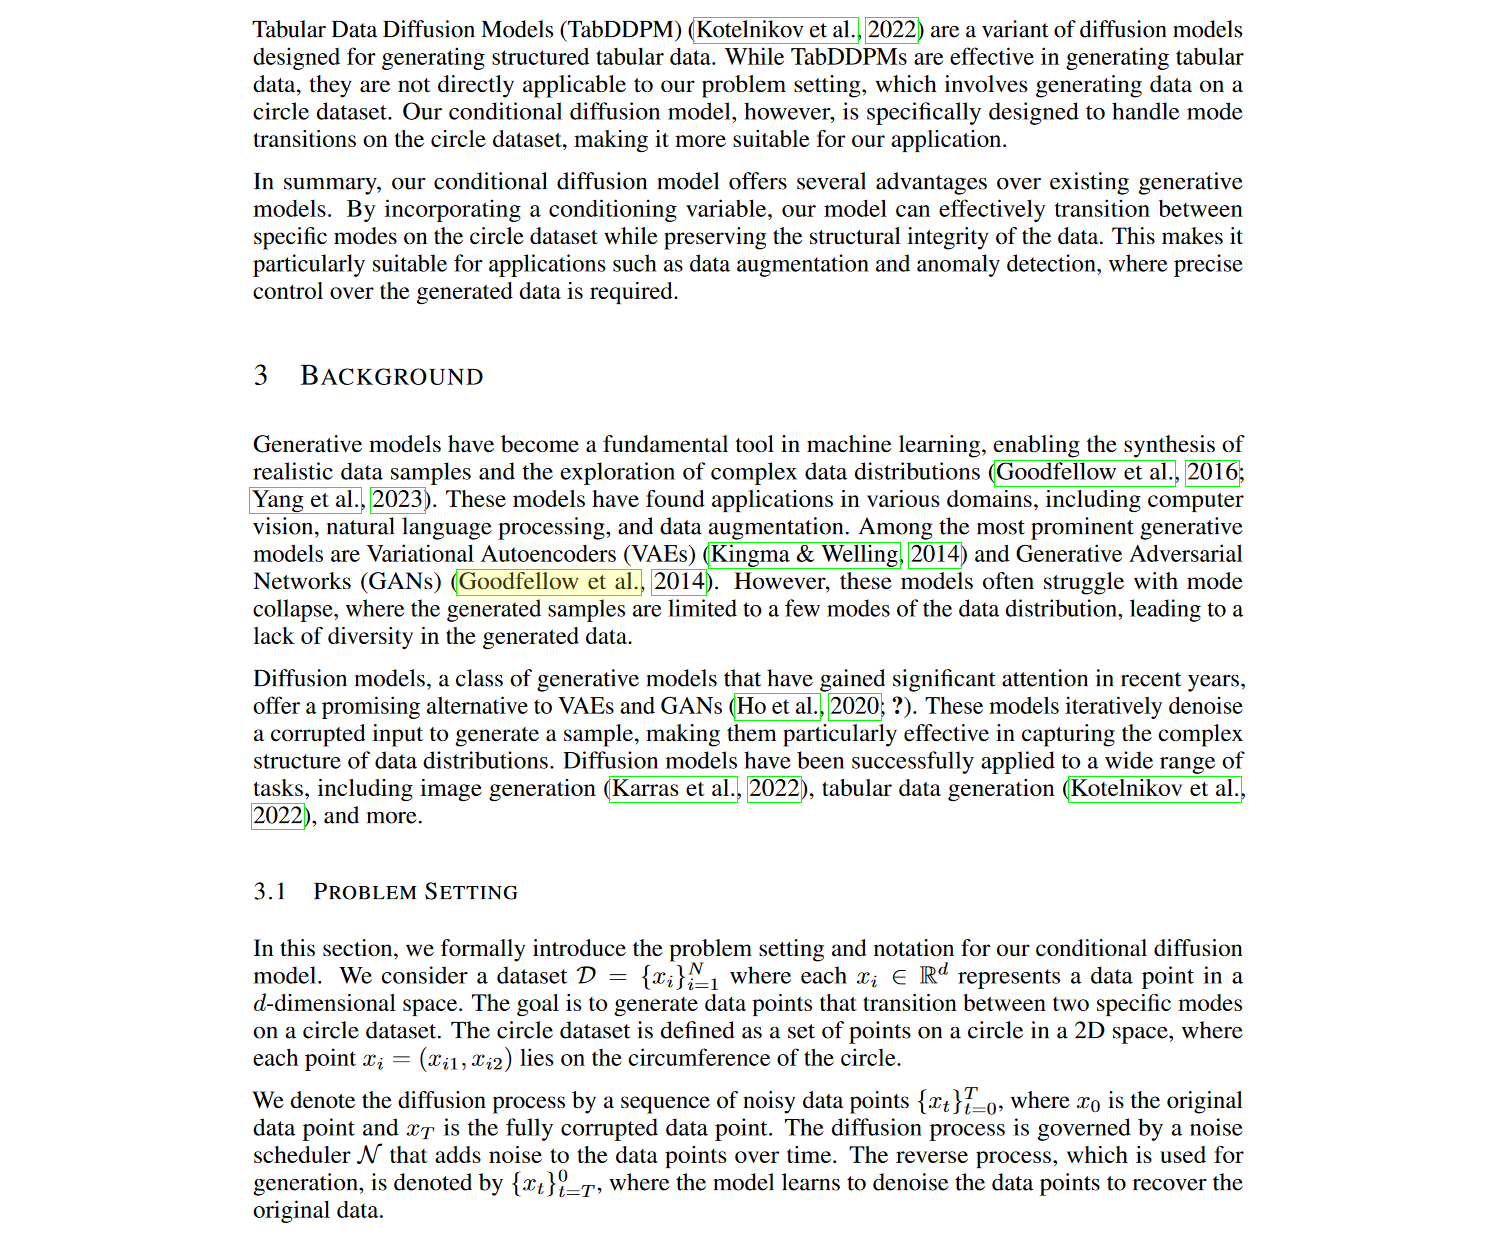
\includegraphics[width=1\textwidth]{images/paper3.png}
    \end{minipage}
    \hfill 
    \begin{minipage}{0.48\textwidth}
        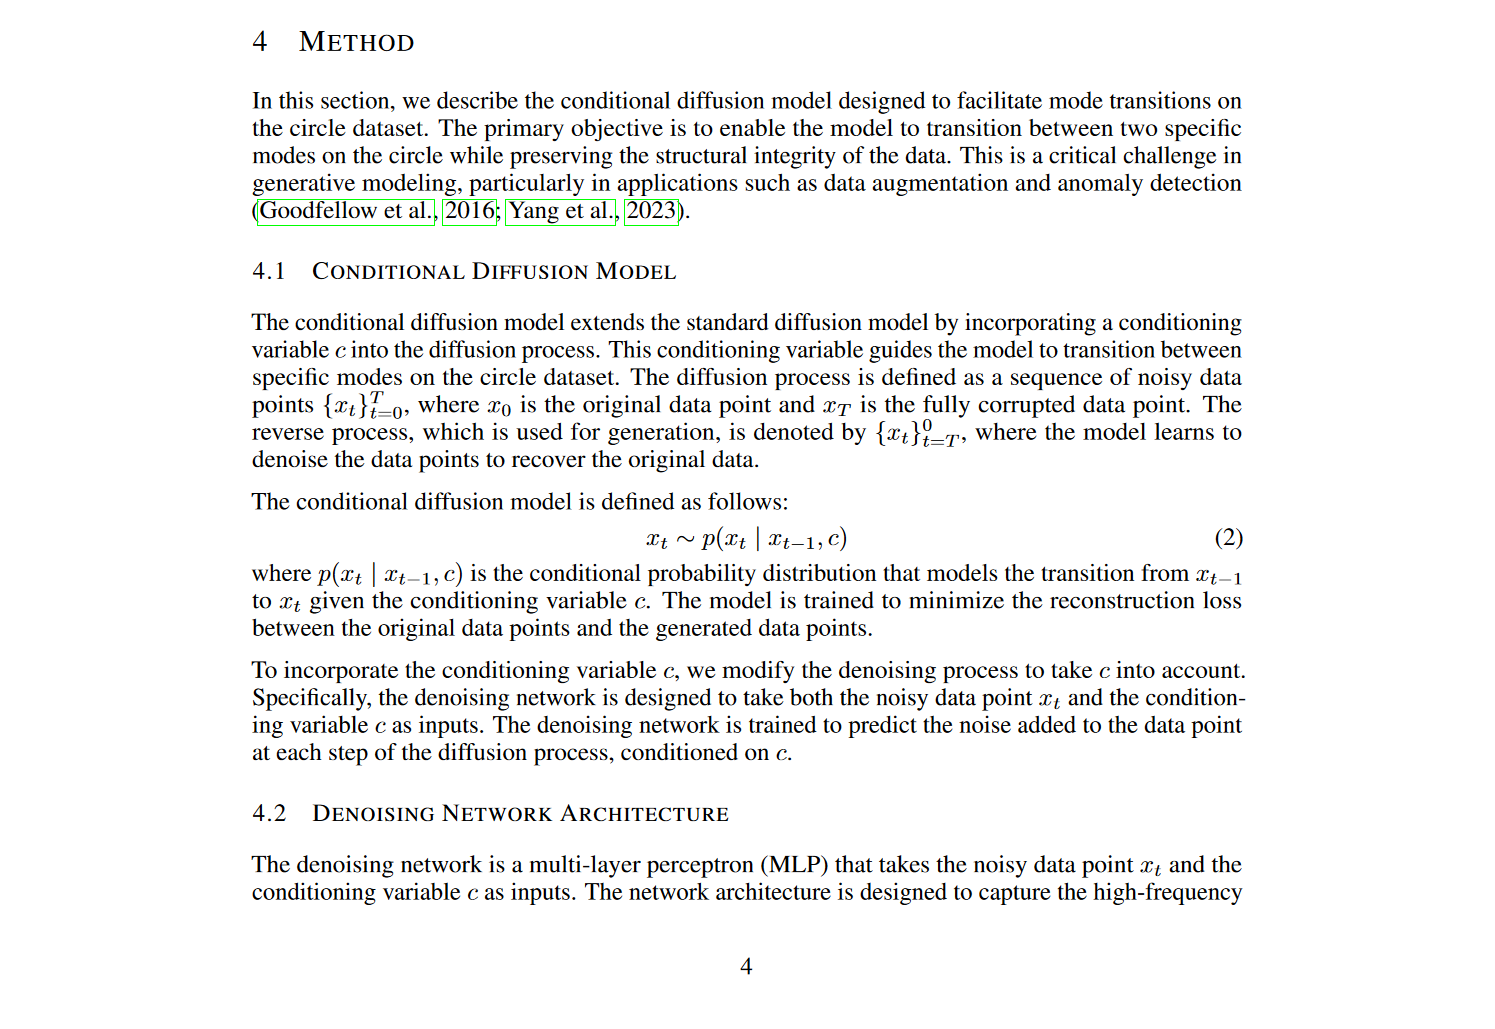
\includegraphics[width=1\textwidth]{images/paper4.png}
    \end{minipage}
    \caption{Visualization of a sample paper generated by the framework}
\end{figure}

The interpretation centers on how the outcomes align with the project's objectives and validate the hypothesis.
\subsection{General Observations}
\begin{itemize}
    \item \textbf{Preservation of Structural Integrity:} The visual representation confirms that the proposed method effectively transitions datasets across modes without sacrificing structural fidelity. For instance, the circle dataset remains circular, while distinct shapes (e.g., ``dino'') retain their recognizability throughout the transformation process.
    \item \textbf{Uniform Transition:} The uniformity observed across all dataset samples suggests that the conditioning variable successfully guided the diffusion process, leading to consistent results across different iterations.
\end{itemize}

\subsection{Comparisons with Established Models}
\begin{itemize}
    \item \textbf{Better Mode Representation:} Compared to Variational Autoencoders (VAEs), the generated results suggest higher reliability in retaining multimodal transitions. This is particularly important as it avoids the common issues of mode collapse often observed in VAE-generated outputs.
    \item \textbf{Efficiency over GANs:} In comparison with Generative Adversarial Networks (GANs), the model's ability to avoid adversarial training pitfalls provides a more stable and scalable approach. This stability is crucial for practical applications.
\end{itemize}

\begin{figure}[t]
    \centering
    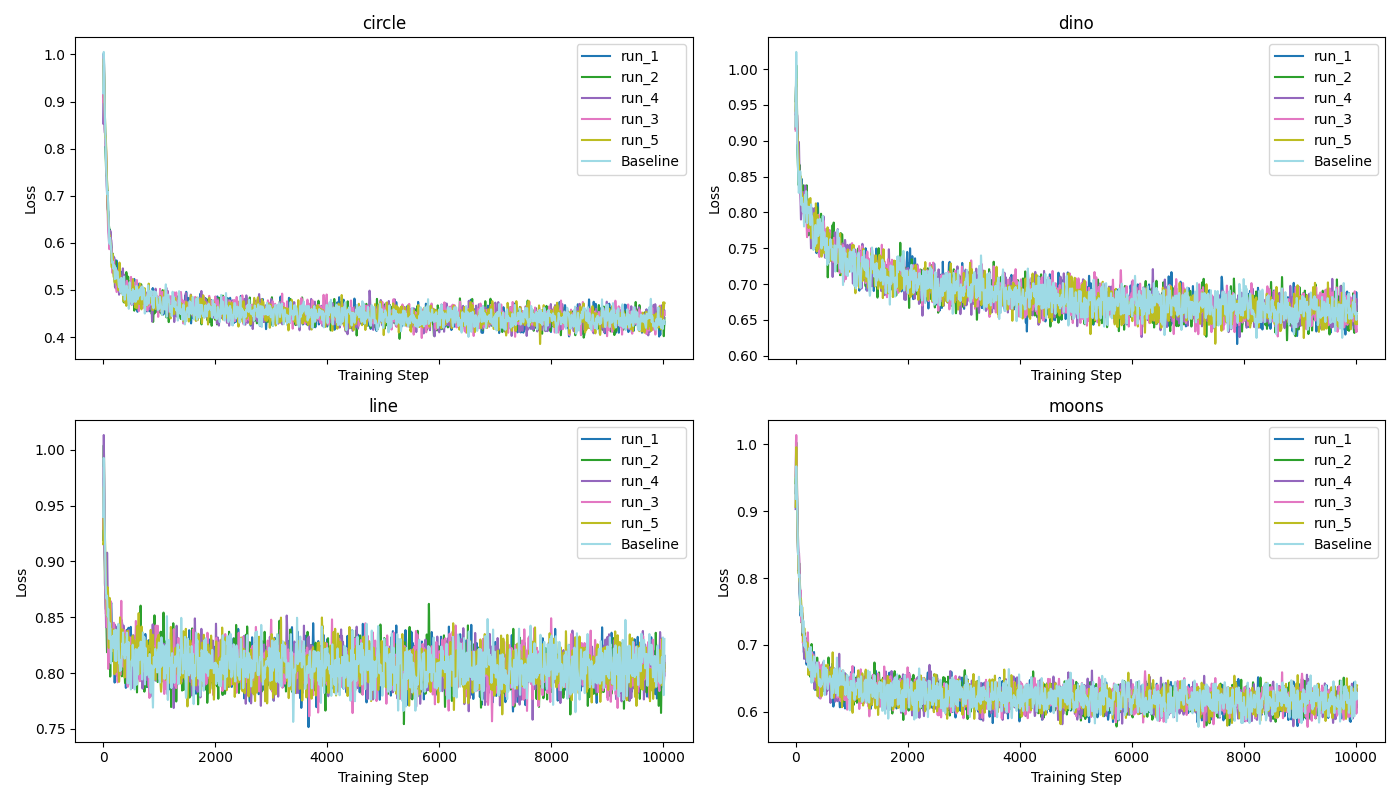
\includegraphics[width=0.8\textwidth, height=0.7\textwidth]{images/train_loss.png}
    \caption{Plots generated by the framework showing training loss over epochs for the generated paper's model.}
    \label{fig:output_b} % chktex 24
\end{figure}

\subsection{Addressing Research Challenges}
\begin{itemize}
    \item \textbf{Mode Collapse:} The results indicate a significant reduction in mode collapse, which is a common challenge faced by generative models. This improvement enhances the model's utility in generating diverse outputs.
    \item \textbf{Anomaly Handling:} The ability to preserve subtle features within datasets—such as those found in the ``moons'' dataset—points to robustness in handling anomalies. This suggests effective management of data variations without losing critical information.
\end{itemize}




% \begin{tcolorbox}[colback=blue!5!white, colframe=blue!75!black, title=Review Summary, ] 
% \textbf{Review Summary:} The paper investigates the impact of data augmentation on the grokking phenomenon in neural networks learning modular arithmetic operations. Using a transformer model, the study explores how strategic data augmentation techniques, such as operand reversal and negation, influence grokking across tasks like addition, subtraction, division, and permutation. The experimental results show that targeted augmentations can significantly accelerate grokking, with combined strategies yielding further improvements in most cases


% \textbf{Strengths:}
% \begin{itemize}
%     \item Addresses a novel and relevant topic in deep learning, focusing on the grokking phenomenon
%     \item Provides a comprehensive analysis of different data augmentation strategies and their effects on grokking dynamics
%     \item Robust experimental setup with multiple runs and conditions tested to ensure reliability
%     \item Findings suggest practical strategies for enhancing model training efficiency and generalization capabilities
% \end{itemize}

% \textbf{Weaknesses:}
% \begin{itemize}
%     \item Lacks clarity in some sections, particularly in the methodology and the detailed implementation of experiments
%     \item Limited discussion on the impact of different augmentation probabilities; more thorough investigation needed
%     \item Results are highly specific to modular arithmetic operations, limiting generalizability to other domains
%     \item Insufficient exploration of how these techniques could be applied to different neural network architectures
%     \item Theoretical justifications for the observed effects are lacking
%     \item Potential ethical concerns regarding the use of data augmentation in critical applications are not addressed
% \end{itemize}
% \end{tcolorbox}

% \begin{tcolorbox}[colback=blue!5!white, colframe=blue!75!black,]
% \textbf{Metrics:}
% \begin{itemize}
%     \item Originality: 3
%     \item Quality: 3
%     \item Clarity: 3
%     \item Significance: 3
%     \item Soundness: 3
%     \item Presentation: 3
%     \item Contribution: 3
%     \item Overall: 5
%     \item Confidence: 4
% \end{itemize}

% \textbf{Questions:}
% \begin{enumerate}
%     \item Can the authors provide more details on the methodology and the specific implementation of experiments?
%     \item How do different augmentation probabilities impact the results across various tasks?
%     \item Can the authors discuss the potential applicability of their findings to different neural network architectures and other domains?
%     \item Can the authors provide a more detailed theoretical explanation for the observed grokking phenomena with data augmentations?
%     \item What steps were taken to ensure the reproducibility of the experiments?
%     \item Can the authors discuss the limitations of their approach and potential negative societal impacts?
%     \item Could the authors elaborate on the reasoning behind the observed improvements in grokking speed due to data augmentations?
%     \item What are the potential ethical concerns of applying these data augmentation strategies in real-world applications?
% \end{enumerate}
% \end{tcolorbox}

% \begin{tcolorbox}[colback=blue!5!white, colframe=blue!75!black, ]
% \textbf{Limitations:}
% \begin{itemize}
%     \item The paper's clarity and thoroughness in discussing methodology and results need improvement
%     \item The generalizability of the findings to other domains and architectures requires further exploration
%     \item The study acknowledges the sensitivity of results to hyperparameters and task specificity. However, it should also consider the broader applicability and potential limitations in real-world scenarios
%     \item Potential negative societal impacts are not discussed, which is important for a comprehensive evaluation of the work
% \end{itemize}

% \textbf{Decision:} Reject

% \textbf{Ethical Concerns:} False
% \end{tcolorbox}

\section{Discussion}
In this project, we introduced a framework designed to fully automate the scientific discovery process, applying it to machine learning itself as a demonstration of its capabilities. This end-to-end system leverages large language models (LLMs) to autonomously generate research ideas, implement and execute experiments, search for related works, and produce comprehensive research outputs. By integrating stages of ideation, experimentation, and iterative refinement, the framework aims to replicate the human scientific process in an automated and scalable manner.\\
Writing projects matters for several reasons. Given our overarching goal to automate scientific discovery, it is crucial for the framework to produce written outputs similar to those of human researchers. First, writing projects offers a highly interpretable method for humans to benefit from the knowledge gained. Second, reviewing written projects within the framework of existing machine learning conferences enables us to standardize evaluation. Third, the scientific project has been the primary medium for disseminating research findings since the dawn of modern science. A project can use natural language and include plots and code, allowing it to flexibly describe any type of scientific study and discovery. Almost any other conceivable format is locked into a certain kind of data or type of science. Until a superior alternative emerges (or possibly invented by AI), we believe that training the framework to produce scientific projects is essential for its integration into the broader scientific community.\\
The framework is remarkably versatile and effectively conducts research across various subfields of machine learning, including transformer-based language modeling, neural network learning dynamics, and diffusion modeling. The cost-effectiveness of the system—producing projects with potential conference relevance at an approximate cost of \$15 per project—highlights its ability to democratize research and accelerate scientific progress. Preliminary qualitative analysis suggests that the generated projects can be broadly informative and novel or at least contain ideas worthy of future study.\\
The actual compute allocated for conducting experiments in this work is also incredibly light by today’s standards. Notably, our experiments generating hundreds of projects were largely run using a single 8×NVIDIA H100 node over the course of a week. Massively scaling the search and filtering would likely result in significantly higher-quality outputs.
In this project, the bulk of the cost associated with running the framework is linked to LLM API costs for coding and project writing. In contrast, costs related to running the LLM reviewer and computational expenses for conducting experiments are negligible due to constraints imposed to keep overall costs down. However, this cost breakdown may change in the future if applied to other scientific fields or used for larger-scale computational experiments.\\
To quantitatively evaluate and improve the generated projects, we created and validated an Automated Project Reviewer. We found that LLMs are capable of producing reasonably accurate reviews, achieving results comparable to humans across various metrics. Applying this evaluator to the outputs generated by the framework enables us to scale evaluation beyond manual inspection.\\
We find that certain models consistently produce high-quality outputs, with some even achieving scores that exceed acceptance thresholds at standard machine learning conferences as judged by our automated reviewer. However, there is no fundamental reason to expect a single model to maintain its lead indefinitely. We anticipate that all frontier LLMs will continue to improve, leading to increased capabilities through competition among them.\\
My work aims to be model-agnostic regarding foundation model providers. In this project, we studied various proprietary LLMs but also explored using open models like DeepSeek and Llama-3. We found that open models offer significant benefits such as lower costs, guaranteed availability, greater transparency, and flexibility, albeit with slightly lower quality. In the future, we aim to use our proposed discovery process to produce self-improving systems in a closed-loop environment using open models.